% This is "www2008-sample.tex" copied from "www2005-sample.tex" V1.2 January 26 2004
% This file should be compiled with V1.4 of "www2008-submission.class"
%
% This example file demonstrates the use of the 'www2008-submission.cls'
% V1.4 LaTeX2e document class file. It is for those submitting
% articles to the WWW'04 Conference WHO DO NOT WISH TO 
% STRICTLY ADHERE TO THE SIGS (PUBS-BOARD-ENDORSED) STYLE.
% The 'www2008-submission.cls' file will produce a similar-looking,
% albeit, 'tighter' paper resulting in, invariably, fewer pages.
%
% ----------------------------------------------------------------------------------------------------------------
% This .tex file (and associated .cls V1.4) produces:
%       1) NO Permission Statement
%       2) WWW'04-specific conference (location) information
%       3) The Copyright Line with ACM data
%       4) NO page numbers
%
% ---------------------------------------------------------------------------------------------------------------
% This .tex source is an example which *does* use
% the .bib file (from which the .bbl file % is produced).
% REMEMBER HOWEVER: After having produced the .bbl file,
% and prior to final submission, you *NEED* to 'insert'
% your .bbl file into your source .tex file so as to provide
% ONE 'self-contained' source file.
%
% ================= IF YOU HAVE QUESTIONS =======================
% Questions regarding the SIGS styles, SIGS policies and
% procedures, Conferences etc. should be sent to
% Julie Goetz (goetz@acm.org) or Adrienne Griscti (griscti@acm.org)
%
% Technical questions only to
% Gerald Murray (murray@acm.org)
% ===============================================================
%
% For tracking purposes - this is V1.2 - January 26 2004
\documentclass{../templates/www2008-submission}

\begin{document}
%
\title{Semantic Mining of Social Online Communities}
%\subtitle{[Extended Abstract]
%\titlenote{A full version of this paper is available as
%\textit{Author's Guide to Preparing ACM SIG Proceedings Using
%\LaTeX$2_\epsilon$\ and BibTeX} at
%\texttt{www.acm.org/eaddress.htm}}}
%
% You need the command \numberofauthors to handle the "boxing"
% and alignment of the authors under the title, and to add
% a section for authors number 4 through n.
%
% Up to the first three authors are aligned under the title;
% use the \alignauthor commands below to handle those names
% and affiliations. Add names, affiliations, addresses for
% additional authors as the argument to \additionalauthors;
% these will be set for you without further effort on your
% part as the last section in the body of your article BEFORE
% References or any Appendices.

\numberofauthors{4}
%
% Put no more than the first THREE authors in the \author command

% NOTE: All authors should be on the first page. For instructions
% for more than 3 authors, see:
% http://www.acm.org/sigs/pubs/proceed/sigfaq.htm#a18

\author{
%
% The command \alignauthor (no curly braces needed) should
% precede each author name, affiliation/snail-mail address and
% e-mail address. Additionally, tag each line of
% affiliation/address with \affaddr, and tag the
%% e-mail address with \email.
\alignauthor Diego Berrueta\\
       \affaddr{Fundaci\'on CTIC}\\
       \affaddr{Gij\'on, Asturias, Spain}\\
       \email{diego.berrueta@fundacionctic.org}
\and
\alignauthor Sergio Fern\'andez\\
       \affaddr{Fundaci\'on CTIC}\\
       \affaddr{Gij\'on, Asturias, Spain}\\
       \email{sergio.fernandez@fundacionctic.org}
\and
\alignauthor Lian Shi\\
       \affaddr{Fundaci\'on CTIC}\\
       \affaddr{Gij\'on, Asturias, Spain}\\
       \email{lian.shi@fundacionctic.org}
}

%\additionalauthors{Additional authors: John Smith (The Th{\o}rv\"{a}ld Group,
%email: {\texttt{jsmith@affiliation.org}}) and Julius P.~Kumquat
%(The Kumquat Consortium, email: {\texttt{jpkumquat@consortium.net}}).}

%\date{5 February 2008}

\maketitle

\begin{abstract}
The Online Communities are a very rich font of collective 
knowledge that are untapped. In this paper we present 
several approaches to mining this kind of communities to 
allow a semantic use of all this information. We focused
in discussion communities, such as discussion forums, blogs
wikis, and mailing lists, but the approach could be also 
applied to other kind of online communities.

FIXME: completar y lucir
\end{abstract}

% A category with only the three required fields
%\category{H.4.m}{Information Systems}{Miscellaneous}
%\category{D.2}{Software}{Software Engineering}
%A category including the fourth, optional field follows...
%\category{D.2.8}{Software Engineering}{Metrics}[complexity measures,
%performance measures]

\keywords{semantic mining, online communities, rdf, xsl}

\section{Introduction}

FIXME

\section{Technologies}

We use an ontology and RDF (Resource Description
Framework~\cite{RDF}) to publish online communities into 
the (Semantic) Web, while retaining the meta-data that were present in 
the messages. Additionally, by doing so, the information can be
merged and linked to other vocabularies, such as FOAF.

DERI Galway leads the development of SIOC (Semantically-Interlinked Online
Communities\footnote{\url{http://sioc-project.org/}}), an ontology that 
provides a vocabulary to interconnect different discussion methods such 
as blogs, web-based forums and mailing lists~\cite{Breslin2006,Breslin2005}.
SIOC is now an official W3C member submission~\cite{Bojars2007}.
SIOC has been used as the core framework to represent information from
online communities in all the work described in this paper.


\section{Approaches}

Since SIOC is a recent specification, its adoption is still low, and
only a few sites export SIOC data. There are a number of techniques
that can be used to bootstrap a network of semantic descriptions from
current social sites. We classify them in two categories:

\begin{itemize}
\item Those which require direct access to the underlying database behind
the social web site are \emph{intrusive techniques}.
\item On the other hand, techniques which do not require direct access to
the database and can operate on resources already published on the web
are \emph{non-intrusive}.
\end{itemize}

We further describe each category in the following paragraphs.

\subsection{Intrusive techniques}

A possible approach to the problem is to add new modules in our
social applications (blogs, bulletin boards, etc) that export
a semantic view (in RDF) of the community. In this way many
developers have written exporters\footnote{\url{http://sioc-project.org/exporters}}
for the most popular Web applications.

This approach is very valid and powerfull, because it has direct 
access to the back-end storage or API of Web applications. Then it
couldn't applied in cases that you haven't access on this kind
of resources. And here is where it apears the other approach to
the problem.

\subsection{Unintrusive techniques}

Another possible approach uses unintrusive techniques. These 
techniques are based in a crawler process that fecthes the data 
published in online communities in (X)HTML. So we don't need to
access to a server-side appliaction to mining the data.

Then different approaches are used to extract the information 
in RDF:

FIXME

\subsubsection{From mboxes to RDF: SWAML}

The first approach uses SWAML~\cite{SWAML2007}. SWAML takes mailing 
list archives in raw format, typically stored in a ``mailbox'' 
(or ``mbox''), as defined in RFC~4155~\cite{RFC4155}. We have 
developed SWAML, a Python script that parses mailboxes and 
outputs RDF descriptions of the messages using the SIOC ontology.
SWAML is a highly configurable, non-interactive application designed 
to be invoked by the system task scheduler.

Some could think that this is a intrusive approarch, becuase it needs
to access on mailboxes to export RDF. But many mailing lists publish
their mailboxes (sometime splited by months or by days) directly by 
HTTP, so it is very easy to fetch (and merge) it. We have tested SWAML 
with the archives of the GNOME project, as we tell later in 
section~\ref{sec:gnome} of this paper. 

FIXMEEE	

\subsubsection{Scraping the HTML archives using XSLT}

Unfortunately, mailing list archives are often unavailable in raw
format. Sometimes we can only access to the ``cooked'' HTML
version of the archives. In such cases, we can use a different
approach: to scrap the data from the HTML file. As each web site
uses a different, customized template for these HTML files, it is
difficult to develop a generic scrapper. We implemented one
for the Debian mailing list archives. It first retrieves all
the relevant files by means of a web crawler. Then it tidies the
markup in order to obtain well-formed XML. During the last stage,
each file is transformed into RDF/XML using XSLT.

Using these approach we have collected \textbf{FIXME} RDF triples
from a selected subset of \textbf{FIXME: number of lists} lists for
the period 2005-2006.

\subsubsection{RDFa enrichement}

Another possible way is to take (X)HTML markup of communities and
enrich it with RDFa~\cite{Birbeck2006}, using XSLT or DOM. The process
generates an output in XHMTL+RDFa that could be easy extracted in RDF 
with one of the parsers available (such as RDFa Distiller\footnote{\url{http://www.w3.org/2007/08/pyRdfa}}).

This approach is quite similar than the aproach used in mle~\cite{Hausenblas2007}
project.


\section{Common problem}

These approaches for mining online communities have some common problem:

\begin{itemize}
  \item \textbf{Identities:} as it can be seen in figure~\ref{fig:foaf-sioc},
	a person (an instance of \texttt{foaf:Person}) can own many online 
	accounts (instances of \texttt{sioc:User}). So we must apply techniques
	(such as Smushing\footnote{\url{http://esw.w3.org/topic/RdfSmushing}})
	in order to extract the real identy behind a online account.

	\begin{figure}[ht]
	 \centering
	 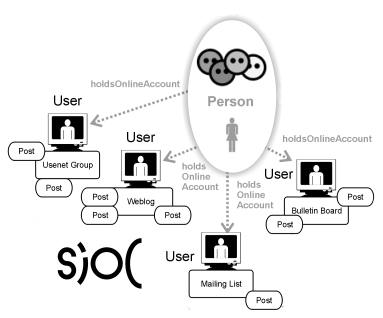
\includegraphics[width=7cm]{images/foaf-sioc.png}
	 \caption{\label{fig:foaf-sioc}Online identity, relationship between FOAF and SIOC}
	\end{figure}

  \item \textbf{Problems with sha1 algorithm:} related with previous problem,
	we detected a problem using sha1 algorithm~\cite{Eastlake2001}. FOAF 
	and SIOC use this algorithm (in properties \texttt{foaf:mbox\_sha1sum} 
	and \texttt{sioc:email\_sha1}, respectively) in order to protect email 
	addresses from SPAM attacks. And this algoritm is case sensitive. So,
	for example, if we take Diego's email address, we could write it as
	\texttt{diego.berrueta@fundacionctic.org} or as \texttt{Diego.Berrueta@fundacionctic.org}.
	Both are valid email addresses. But each one generates different sha1sum.
	This could  seem a detail without importance, but it really creates a 
	serious problem when try to identify persons/users using these
	inverse functional properties. Unfortunately in our experimientos we 
	have found many times this kind of problem.

  \item \textbf{\textit{Flat} thread:} FIXME

  \item \textbf{Repeated keys:} FIXME

  \item \textbf{Paginated discussions:} FIXME


\end{itemize}


\section{Experimentation with Free Sofware communities}

FIXME

\section{\label{sec:gnome}GNOME mailing lists}

GNOME project publishes archives of its mailing lists~\footnote{\url{http://mail.gnome.org/archives/}}.
It is an archive with around 200 mailing list with information of 
more than ten years of activity in the project. Fortunately these
archives are not only published in (X)HTML, but also there are 
available (gzipped) mailboxes for each month. So we wrotte a simple
crawler to fetch these raw data directly by HTTP, and merge archive
of each month in a single mailbox for each mailing list of the project.

Then we had all necessary information to start running SWAML on these 
more than 200 mailboxes. For a selected subset of the mailing lists, 
SWAML has produced plus 25 million triples.

\section{Debian mailing lists}

FIXME

\section{Ubuntu Forums}

Ubuntu Forums\footnote{\url{http://ubuntuforums.org/}} are a very popular 
discussion forusm among users of this GNU/Linux distribution. They have a 
frenetic activity, with plus than 4 million of posts in the moment we made
our experiments.

In these forums we used a quite similar appoach than with Debian mailing
lists. We analized the markup generated by vBulletin (CMS used in these forums)
and we developed some XSLT stylesheets to transform get instances of
\texttt{sioc:Forum}, \texttt{sioc:Thread} and \texttt{sioc:Post}. We 
selected only a subset of available forums to test our application, FIXME

\section{Advogato}

FIXME


\section{\label{sec:conclusions}Conclusions}

Semantic descriptions of online communities pushes them
into a new level of functionality. On the one hand, they can be
conveniently browsed and queried. Search engines can exploit the
metadata to improve their precission, and at the same time, to
avoid repeated results.

On the other hand, the semantic descriptions can be
analysed and mined. Futhermore, they can be linked to other resources,
thus reducing the risk of creating an ``information silo'' and
enabling the rise of a network of ``linked data''.

So far, no semantic annotation relative to the meaning of
the messages is considered. Obviously, it is very difficult
to extract such information from the message text.
However, it is conceivable that it can be added by other 
means, such as social tagging using folksonomies, or parsing the 
RDFa that may exist in the e-mail messages that are send in XHTML 
format.The inherent community-based nature of mailing lists can
be exploited to build recommendation systems~\cite{Celma2006}.

FIXME

\section*{Acknowledgements}

FIXME


% The following two commands are all you need in the
% initial runs of your .tex file to
% produce the bibliography for the citations in your paper.
\bibliographystyle{abbrv}
\bibliography{../references}

\balancecolumns

\end{document}
